\chapter{Implementación}
\label{capitulo5}
\section{Aspectos Generales}
En esta sección se presentan las herramientas y metodologías elegidas para realizar la implementación de la herramienta.

\subsection{Entorno de desarrollo}
El entorno desarrollado durante la implementación del sistema y desarrollo del caso de estudio:

\begin{itemize}
	\item Sistemas operativos: Mac OS 10.9.3 (Maverick) y Linux Mint 15
	\item Sistemas operativos utilizados en el testeo y caso de estudio: Linux Mint 15
	\item Lenguajes de desarrollo: Perl y Python (web framework Django)
	\item Entorno de desarrollo: vim\footnote{Vim es un editor de texto que está diseñado para usarse tanto desde una interfaz de línea de comandos o como una aplicación independiente en una interfaz gráfica de usuario.}  con plugins provistos por spf13\footnote{http://vim.spf13.com/ centraliza un conjunto de plugins para vim.}
	\item Base de datos: Mysql versión 14.14 distribución 5.5.34
	\item Sistema de versionado: git
	\item Servidor web: apache2
	\item Versión de RT: RT4
	\item Testeo de APIs Rest: Postman\footnote{Es una herramienta de chrome utilizada para probar, desarrollar y documentar APIs.}
	
\end{itemize}

\subsection{Metodología}
Para la implementación de la herramienta se debió utilizar el lenguaje de programación PERL para el desarrollo de un plugin para la herramienta RT.\\
	\bigskip
Se utilizó el framework web Django por permitir desarrollar aplicaciones web de forma rápida y con la escritura de poco código. Además busca automatizar parte del desarrollo al basarse en el principio DRY (\textit{Don’t Repeat Yourself}). Presenta la ventaja de utilizar el patrón de arquitectura MVC (\textit{Model View Controller}). La ventaja de utilizar este patrón es que divide la aplicación en tres partes interconectadas y da una base inicial con la cual desarrollar el trabajo. A su vez, utilizar un patrón MVC presenta la ventaja de que se tiene experiencia desarrollando aplicaciones utilizando dicho patrón lo cual facilita el trabajo.
La existencia de librerías implementadas en python para trabajar con STIX y TAXII influyo fuertemente en la decisión de utilizar Django. Otra de las razones fue la existencia de una implementación de referencia con la cual se puede testear el desarrollo realizado.\\
	\bigskip
La metodología utilizada fue la de un desarrollo incremental, esto permitió realizar una validación de la arquitectura propuesta. Luego de realizar dicha validación se siguió implementando la herramienta propuesta.

\subsection{Librerias utilizadas}
Durante el transcurso de la implementación se utilizaron distintas librerías Perl y Python para el desarrollo de la herramienta.

\subsubsection{Django Rest Framework}
Es una librería para Django que hace simple el construir APIs REST de forma sencilla y rápida. La librería se utilizó para implementar la API REST que se consume desde el plugin RT-TAXII, dicho plugin se explicará mas adelante.

\subsubsection{LWP}
LWP se refiere a LibWww-Perl y es un conjunto de módulos Perl que proveen una API simple para desarrollar clientes web y desarrollar servidores http. En particular se utilizó el módulo LWP::UserAgent que permite realizar con facilidad pedidos web.
Con esta librería se realizan los pedidos que se hacen a la componente  libTAXII.

\subsubsection{libTAXII}
Es una librería Python para manejar mensajes TAXII e invocar servicios TAXII. Uno de sus objetivos es ser fiel a las especificaciones de TAXII y a las buenas prácticas de Python.
La librería provee:

\begin{enumerate}
	\item
	Una representación de objetos de los mensajes TAXII.
	\item
	Permite transformar XML en objetos Python y viceversa.
	\item
	Un cliente HTTP/HTTPS TAXII.
\end{enumerate}

Esas tres características se utilizaron durante el desarrollo de la herramienta. Debido a que primero se crea un objeto Python que representa el mensaje TAXII, dicho objeto es transformado a XML para ser enviado por el cliente TAXII, la respuesta al mensaje enviado también es un objeto XML, dicho XML es transformado a un objeto Python para ser procesado.
A su vez cuando se recibe un XML, este se transforma a un objeto Python para ser procesado, luego del procesamiento se devuelve una respuesta XML por medio del cliente HTTP/HTTPS.

\subsubsection{pythonStix}
Es una librería Python que provee una API para parsear, manipular y consumir contenido STIX. Los desarrolladores pueden utilizar la API para desarrollar aplicaciones que crean, consumen, traducen o procesen contenido STIX.
Se utilizo en taxiiApp para crear paquetes STIX a partir de un cyber observable que ingrese el usuario en RTIR. Además durante los intercambios se obtiene información de los paquetes STIX para lo cual es necesario parsear la información del paquete STIX. 


\subsubsection{YETI}
YETI es una prueba de concepto de TAXII creado para ayudar a los desarrolladores a implementar y testear sus propias aplicaciones TAXII. A su vez ayuda a aprender más sobre el funcionamiento de TAXII.
Fue utilizada en etapas tempranas del proyecto como referencia y para testear el desarrollo realizado. De esta forma mientras se avanzó en el desarrollo se pudo validar de forma adecuada que se respetara adecuadamente la especificación de TAXII.

\subsection{Módulos desarrollados}
A continuación se describen lo módulos implementados para el funcionamiento de la herramienta, así como las consideraciones necesarias para extender la herramienta con nuevas funcionalidades.

\subsubsection{RT-TAXII}
Se desarrolló un plugin para RTIR que es el encargado de consumir la API rest provista por TAXIIApp y que extiende la interfaz web de RTIR para presentarle al usuario los formularios necesarios para que interactúe con el sistema.
Se incluyó en el menú de RTIR una nueva sección en la que se especifican las distintas acciones que se pueden realizar referentes a TAXII.
Cada una de estas acciones invoca a un script desarrollado en PERL que presenta el formulario al usuario.
Luego de que el usuario ingresa la información deseada y realiza el envío de la información. El sistema invoca a la API Rest provista por TAXII App.
Es necesario que se configure la dirección del host en la que se encuentra ejecutando TAXIIApp.
La estructura de directorios de RT-TAXII es la que se muestra en la figura \ref{fig.rt_taxii}.\\

\begin{figure}[h!]
	\centering
	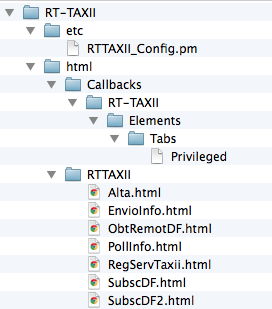
\includegraphics{imagenes/RT-TAXII.png}
	\caption{Estructura de directorios de plugin RT-TAXII}
	\label{fig.rt_taxii}
\end{figure}
	\bigskip
El archivo RTTAXII\_Config.pm es utilizado para guardar las configuraciones del plugin. Dentro de dichas configuraciones se encuentran parámetros necesarios para el funcionamiento del sistema.
En el archivo Privileged se realiza la configuración del menú que contiene las funcionalidades del sistema.
Los archivos incluidos en el directorio RTTAXII son los encargados de presentar los formularios y realizar la lógica correspondiente a las llamadas a TAXIIApp. Dichos archivos están implementados en PERL y contienen HTML para realizar la presentación al usuario.\\

Para extender la herramienta con nuevas funcionalidades es necesario crear un nuevo script PERL en el directorio RTTAXII. Dicho script debe implementar las funcionalidades que se deseen. Como RT está desarrollado en PERL se cuenta con todos los módulos disponibles de PERL.

\subsubsection{TAXIIApp}
A continuación se describirán los componentes implementados y como estos interactúan con las librerías utilizadas.
También se mencionarán las consideraciones que se deben tener para expandir la herramienta.
En la figura \ref{fig.taxii_app} se ven los distintos módulos implementados durante el proyecto. 

\begin{figure}
	\centering
	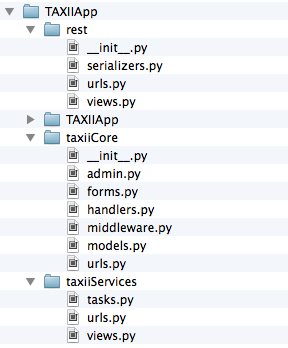
\includegraphics{imagenes/TAXIIApp.png}
	\caption{Aplicación TAXII implementada junto con sus módulos}
	\label{fig.taxii_app}
\end{figure}

\paragraph{TAXIICore}\ \\
TAXII Core es la componente encargada del procesamiento de la información, es invocada por la API Rest y por TAXII Services y actúa dependiendo de la información recibida. Además es la encargada de la comunicación con la base de datos por medio del modelo de datos desarrollado. A su vez se tuvo consideración durante el desarrollo que este componente sería el encargado de dialogar con los módulos de sanitización y correlación de información. 
En el anexo se pueden ver las entidades creadas para modelar la base de datos así como los métodos implementados para enviar y recibir información del resto de las componentes.

\paragraph{TAXIIServices}\ \\
Este módulo es el encargado de la comunicación con otra organización por medio del protocolo TAXII. Se desarrollaron  los distintos métodos necesarios para implementar los servicios TAXII exceptuando el discovery service.
Se utiliza libTAXII para crear los mensajes a intercambiar y para realizar la invocación a los servicios de otras organizaciones.
Los mensajes luego de recibidos son pasados a TAXIICore para su procesamiento.
En caso de que se crearan nuevos servicios o que se quisiera implementar por ejemplo el discovery service esto se realizaría en este módulo.
En el anexo se pueden ver las firmas de los servicios implementados.

\paragraph{REST API}\ \\
La API Rest desarrollada provee las funcionalidades necesarias para que RT-TAXII interactúe con TAXII App. Dentro de dichas interacciones se permite el manejo de cualquiera de los elementos del modelo en TAXIICore. Además se crearon métodos específicos para el uso de TAXII. Se permite el envío y poll de información, obtención de data feeds así como la subscripción a estos.\\

Para la implementación se utilizo la librería auxiliar \textit{Django Rest framework} que simplifica el desarrollo de la API.
Si bien se implementaron todos los elementos necesarios para realizar la interacción con la base de datos, si existiera un cambio en esta (i.e: se crea una nueva entidad) sería necesario extender esta API para poder realizar la interacción entre los sistemas. A su vez si se crea un nuevo servicio TAXII y se desea proveer una interfaz en RTIR para que los usuarios interactúen con esta sería necesario agregar los métodos necesarios en esta API.
En el anexo se puede ver la firma de la API desarrollada.
